\section{Đại cương về dòng điện xoay chiều}
\subsection{Tóm tắt lí thuyết}
\begin{tomtat}
\subsubsection{Nguyên tắc tạo ra dòng điện xoay chiều}
\begin{minipage}{0.5\textwidth}
	Xét khung dây ABCD diện tích $S$, được đặt trong từ trường đều và quay đều với tốc độ góc $\omega$ quay trục $\Delta$. Khi đó, từ thông qua khung dây được xác định bởi:
	\begin{equation}
		\Phi=BS\cos\alpha
	\end{equation}
	Do khung dây quay đều với tốc độ góc $\omega$ nên $\alpha=\omega t+\varphi_0$, và tổng quát hoá cho khung dây có $N$ vòng dây thì ta thu được biểu thức của $\Phi\left(t\right)$:
	\begin{equation}
		\Phi\left(t\right)=NBS\cos\left(\omega t+\varphi_0\right)
	\end{equation}
\end{minipage}
\hfill
\begin{minipage}{0.5\textwidth}
	\centering
	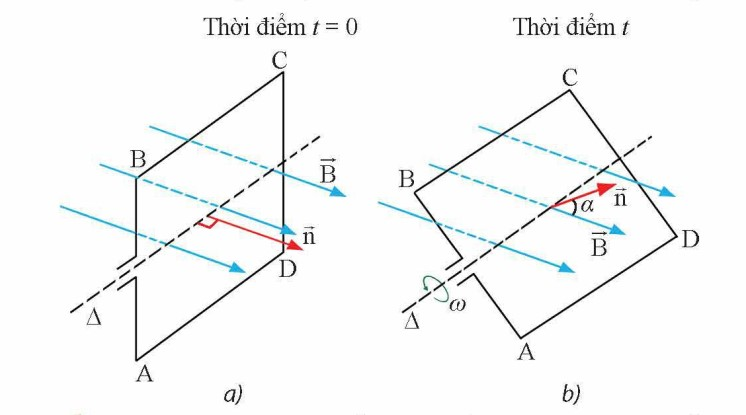
\includegraphics[width=1\linewidth]{figs/VN12-Y24-PH-SYL-023-1}
	\captionof{figure}{Khung dây quay đều trong từ trường.}
\end{minipage}
Theo định luật Faraday, suất điện động cảm ứng tại thời điểm $t$ được xác định:
\begin{equation}
	e\left(t\right)=-\dfrac{d\Phi}{dt}=\omega NBS\sin\left(\omega t+\varphi_0\right)=\omega NBS\cos\left(\omega t+\varphi_0-\dfrac{\pi}{2}\right)
\end{equation}
Suất điện động cảm ứng trong khung dây biến đổi điều hoà theo thời gian và được gọi là \textbf{suất điện động xoay chiều}:
\begin{equation}
	e\left(t\right)=\omega NBS\cos\left(\omega t+\varphi_{0e}\right)=E_0\cos\left(\omega t+\varphi_{0e}\right)
\end{equation}
trong đó $E_0=\omega NBS$ được gọi là suất điện động cực đại.
\begin{center}
	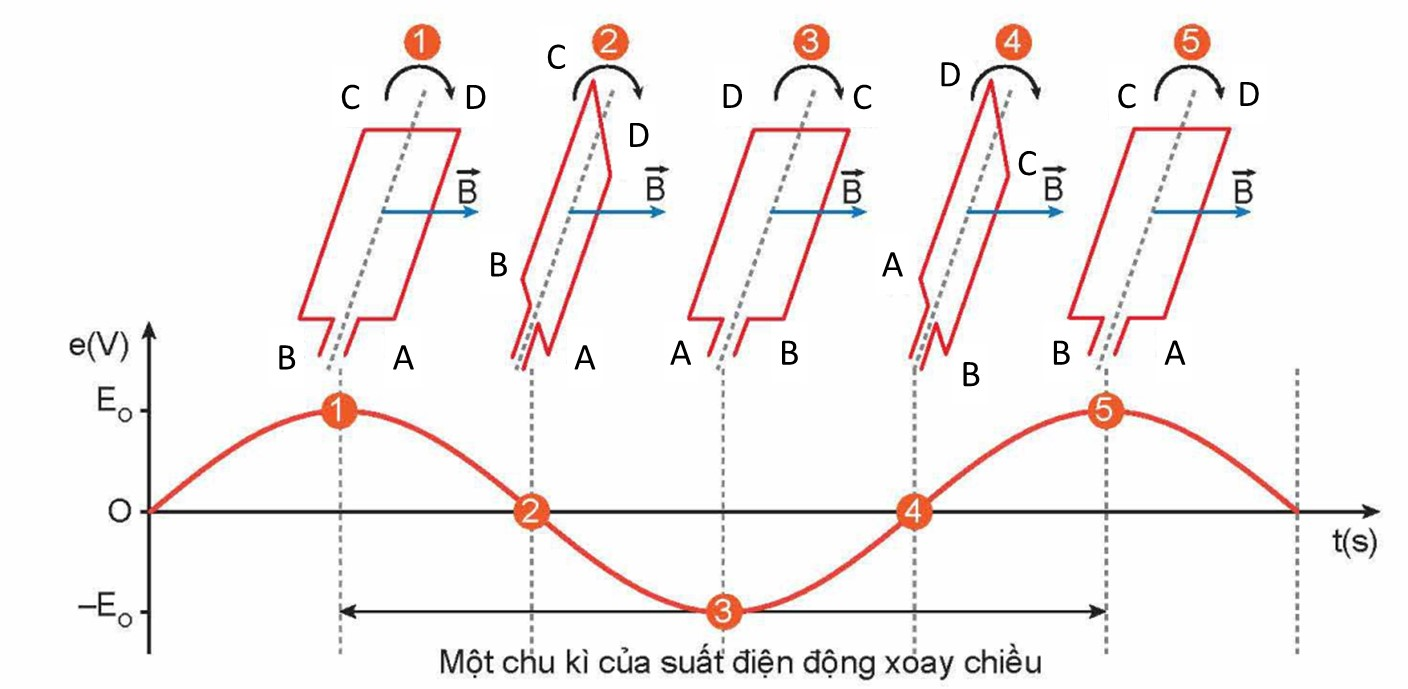
\includegraphics[width=0.8\linewidth]{figs/VN12-Y24-PH-SYL-023-2}
	\captionof{figure}{Mô tả suất điện động xoay chiều khi khung dây quay trong từ trường đều.}
\end{center}
\begin{luuy}
	Có 2 cách tạo ra suất điện động xoay chiều trong các máy điện:
	\begin{itemize}
		\item Từ trường cố định, các vòng dây quay quanh từ trường.
		\item Từ trường quay, các vòng dây đặt cố định.
	\end{itemize}
\end{luuy}
\subsubsection{Dòng điện xoay chiều}
Khi nối mạch tiêu thụ vào điện áp xoay chiều $u=U_0\cos\left(\omega t+\varphi_{u}\right)$ thì trong mạch có dòng điện xoay chiều $i=I_0\cos\left(\omega t+\varphi_{i}\right)$.\\
\begin{dn}
	Dòng điện xoay chiều là dòng điện có cường độ biến thiên điều hoà theo thời gian.
\end{dn}
Trong đó:
\begin{itemize}
	\item $\omega$ là tần số góc của dòng điện xoay chiều, bằng tần số góc của suất điện động cảm ứng do máy phát điện xoay chiều tạo ra, đơn vị trong hệ SI là radian/giây $\left(\si{\radian/\second}\right)$;
	\item $u$ và $i$ là giá trị tức thời của điện áp giữa hai đầu đoạn mạch và cường độ dòng điện trong mạch, đơn vị trong hệ SI lần lượt là volt $\left(\si{\volt}\right)$ và ampere $\left(\si{\ampere}\right)$;
	\item $U_0$ và $I_0$ là giá trị cực đại của điện áp và cường độ dòng điện xoay chiều trong đoạn mạch;
	\item $\varphi_u$ và $\varphi_i$ là pha ban đầu của điện áp và cường độ dòng điện xoay chiều, đơn vị trong hệ SI là radian $\left(\si{\radian}\right)$.
\end{itemize}
\subsubsection{Các giá trị hiệu dụng của dòng điện xoay chiều}
\begin{dn}
	Giá trị hiệu dụng của cường độ dòng điện xoay chiều bằng cường độ của dòng điện không đổi, nếu cho hai dòng điện này lần lượt đi qua cùng một điện trở thì nhiệt lượng toả ra trong thời gian đủ dài là bằng nhau
	\begin{equation}
		I=\dfrac{I_0}{\sqrt{2}}.
	\end{equation}
\end{dn}
Ngoài ra, người ta cũng định nghĩa giá trị hiệu dụng của điện áp xoay chiều ở hai đầu đoạn mạch là
\begin{equation}
	U=\dfrac{U_0}{\sqrt{2}}.
\end{equation}
và suất điện động hiệu dụng của nguồn điện là
\begin{equation}
	E=\dfrac{E_0}{\sqrt{2}}.
\end{equation}
\subsubsection{Sử dụng dòng điện xoay chiều}
\paragraph{Tác dụng và ứng dụng của dòng điện xoay chiều}
\begin{enumerate}[label=\alph*.]
	\item Tác dụng:
	\begin{itemize}
		\item Tác dụng quang (phát sáng);
		\item Tác dụng từ;
		\item Tác dụng nhiệt;
		\item Tác dụng hoá;
		\item Tác dụng sinh lí.
	\end{itemize}
	\item Ứng dụng:
	\begin{itemize}
		\item Các loại đèn thắp sáng, \dots;
		\item Lò luyện kim, mỏ hàn, các động cơ điện, \dots;
		\item Các thiết bị điện gia đình: bàn là, quạt điện, tủ lạnh, \dots;
		\item Hệ thống lưới điện quốc gia là hệ thống lưới điện xoay chiều;
		\item Dòng điện xoay chiều có thể chỉnh lưu thành dòng điện một chiều;
		\item Dòng điện xoay chiều dễ truyền đi xa nhờ dùng máy biến áp.
	\end{itemize}
\end{enumerate}
\paragraph{Quy tắc an toàn khi sử dụng điện xoay chiều}
\begin{itemize}
	\item Dùng các thiết bị điện phù hợp và có chất lượng tốt;
	\item Tuân thủ các biển báo an toàn điện;
	\item Dùng thiết bị tự động ngắt điện (phù hợp với công suất) khi xảy ra chập điện hay quá tải;
	\item Các vị trí lắp đặt ổ cắm điện, cầu dao điện, \dots phải ở nơi khô ráo và tránh xa tầm tay trẻ em (ở trên cao);
	\item Thường xuyên kiểm tra mạng điện, bảo trì các thiết bị điện đúng kì hạn để phát hiện các trường hợp hư hỏng và kịp thời sửa chữa, tránh sự cố xảy ra.
\end{itemize}
\end{tomtat}
\subsection{Ví dụ minh hoạ}
\begin{dang}{Xác định các đại lượng đặc trưng của dòng điện xoay chiều}
	\end{dang}
\begin{vd}
Điện áp của một nguồn điện xoay chiều được cho bởi biểu thức: 
$$\xsi{u=220\sqrt{2}\cos\left(100\pi t+\dfrac{\pi}{3}\right)}{\volt}$$
Hãy xác định:
\begin{enumerate}[label=\alph*)]
	\item giá trị cực đại của điện áp.
	\item giá trị hiệu dụng của điện áp.
	\item tần số của điện áp.
\end{enumerate}
\loigiai{
\begin{enumerate}[label=\alph*)]
	\item Giá trị cực đại của điện áp $U_0=\xsi{220\sqrt{2}}{\volt}\approx\SI{311.12}{\volt}.$
	\item Giá trị hiệu dụng của điện áp 
	$$U=\dfrac{U_0}{\sqrt{2}}=\SI{220}{\volt}.$$
	\item Tần số của điện áp
	$$f=\dfrac{\omega}{2\pi}=\dfrac{\xsi{100\pi}{\radian/\second}}{2\pi}=\SI{50}{\hertz}.$$
\end{enumerate}	
}
\end{vd}
% ==============================================================================
\begin{vd}
Dòng điện xoay chiều được cho bởi biểu thức $i=\xsi{10\sin\left(50\pi t\right)}{\ampere}$. Tính công suất trung bình do dòng điện  tạo ra trên điện trở $\SI{10}{\ohm}$.
\loigiai{
Cường độ hiệu dụng:
$$I=\dfrac{I_0}{\sqrt{2}}=\xsi{5\sqrt{2}}{\ampere}.$$
Công suất trung bình do dòng điện toả ra trên điện trở:
$$\calP=I^2R=\left(\xsi{5\sqrt{2}}{\ampere}\right)^2\cdot\left(\SI{10}{\ohm}\right)=\SI{500}{\watt}.$$	
}
\end{vd}
% =========================================
\begin{vd}
Một ấm điện đun nước hoạt động từ nguồn điện xoay chiều có giá trị điện áp hiệu dụng $\SI{220}{\volt}$, cường độ dòng điện hiệu dụng là $\SI{5.5}{\ampere}$. Tính: 
\begin{enumerate}[label=\alph*)]
	\item điện trở của ấm đun nước.
	\item công suất toả nhiệt của bếp.
\end{enumerate}
Coi ấm đun nước chỉ có điện trở thuần.
\loigiai{
\begin{enumerate}[label=\alph*)]
	\item Điện trở của ấm đun nước:
	$$R=\dfrac{U}{I}=\dfrac{\SI{220}{\volt}}{\SI{5.5}{\ampere}}=\SI{40}{\ohm}.$$
	\item Công suất toả nhiệt của bếp:
	$$\calP=UI=\SI{1210}{\watt}.$$
\end{enumerate}	
}
\end{vd}
\begin{dang}{Mối liên hệ về pha giữa điện áp $u$ và cường độ dòng điện $i$ trong mạch điện xoay chiều}
		Gọi $\varphi=\left|\varphi_u-\varphi_i\right|	$ là độ lệch pha giữa $u$ và $i$.
		\begin{itemize}
			\item Khi $u$ và $i$ cùng pha $\left(\varphi=k2\pi,\ k\in \mathbb{Z}\right)$ thì
			$$\dfrac{u}{U_0}=\dfrac{i}{I_0}.$$
			\item Khi $u$ và $i$ ngược pha $\left(\varphi=\left(2k+1\right)\pi,\ k\in \mathbb{Z}\right)$ thì
			$$\dfrac{u}{U_0}=-\dfrac{i}{I_0}.$$
			\item Khi $u$ và $i$ vuông pha $\left(\varphi=\dfrac{\pi}{2}+k\pi,\ k\in \mathbb{Z}\right)$ thì
			$$\left(\dfrac{u}{U_0}\right)^2+\left(\dfrac{i}{I_0}\right)^2=1.$$
		\end{itemize}
\end{dang}
\begin{vd}
Dòng điện chạy qua đoạn mạch xoay chiều có cường độ $i=\xsi{200\cos\left(100\pi t\right)}{\ampere}$, điện áp giữa hai đầu đoạn mạch có giá trị hiệu dụng là $\SI{12}{\volt}$ và sớm pha $\xsi{\dfrac{\pi}{3}}{\radian}$ so với cường độ dòng điện.
\begin{enumerate}[label=\alph*)]
	\item Tính chu kì, tần số của dòng điện.
	\item Tính giá trị hiệu dụng của cường độ dòng điện trong mạch.
	\item Tính giá trị tức thời của cường độ dòng điện ở thời điểm $t=\SI{0.5}{\second}$.
	\item Trong một giây, dòng điện đổi chiều bao nhiêu lần?
	\item Viết biểu thức của điện áp giữa hai đầu đoạn mạch.
\end{enumerate}
\loigiai{
\begin{enumerate}[label=\alph*)]
	\item Tốc độ góc của dòng điện $\omega=\xsi{100\pi}{\radian/\second}$.\\
	Từ đó, ta có chu kì và tần số của dòng điện là
	\begin{align*}
		\begin{cases}
			T=\dfrac{2\pi}{\omega}=\xsi{\dfrac{1}{50}}{\second}\\
			\ \\
			f=\dfrac{\omega}{2\pi}=\SI{50}{\hertz}
		\end{cases}
	\end{align*}
	\item Giá trị hiệu dụng của dòng điện trong mạch là $I=\dfrac{I_0}{\sqrt{2}}=\xsi{100\sqrt{2}}{\ampere}.$
	\item Tại thời điểm $t=\SI{0.5}{\second}$ thì $i=200\cos\left(100\pi\cdot0,5\right)=\SI{200}{\ampere}$.
	\item Tần số của dòng điện là $f=\SI{50}{\hertz}$, đồng nghĩa là trong một giây thì dòng điện thực hiện được 50 dao động. Do mỗi dao động thì dòng điện đổi chiều 2 lần nên trong một giây dòng điện đổi chiều 100 lần.
	\item Do điện áp sớm pha $\xsi{\dfrac{\pi}{3}}{\radian}$ so với dòng điện nên $\varphi_u=\varphi_i+\dfrac{\pi}{3}=\xsi{\dfrac{\pi}{3}}{\radian}$.\\
	Điện áp cực đại: $U_0=U\sqrt{2}=\xsi{12\sqrt{2}}{\volt}$.\\
	Biểu thức của điện áp hai đầu mạch điện: $u=\xsi{12\sqrt{2}\cos\left(100\pi t+\dfrac{\pi}{3}\right)}{\volt}.$
\end{enumerate}	
}
\end{vd}
% ====================================
\begin{vd}
Một mạch điện xoay chiều có độ lệch pha giữa điện áp và cường độ dòng điện chạy trong mạch là $\xsi{\dfrac{\pi}{2}}{\radian}$. Tại một thời điểm $t$, cường độ dòng điện có giá trị $\xsi{2\sqrt{3}}{\ampere}$ thì điện áp giữa hai đầu mạch là $\xsi{50\sqrt{2}}{\volt}$. Biết điện áp  hiệu dụng của mạch là $\SI{100}{\volt}$. Tính giá trị hiệu dụng của cường độ dòng điện chạy qua mạch.
\loigiai{
Do điện áp và cường độ dòng điện vuông pha nên
$$\left(\dfrac{u}{U_0}\right)^2+\left(\dfrac{i}{I_0}\right)^2=1.$$
Thay các giá trị:
\begin{align*}
	\begin{cases}
		i=\xsi{2\sqrt{3}}{\ampere}\\
		u=\xsi{50\sqrt{2}}{\volt}\\
		U=\SI{100}{\volt}\Rightarrow U_0=\xsi{100\sqrt{2}}{\volt}
	\end{cases}
	\Rightarrow \left(\dfrac{50\sqrt{2}}{100\sqrt{2}}\right)^2+\left(\dfrac{2\sqrt{3}}{I_0}\right)=1\Rightarrow I_0=\SI{4}{\ampere}.
\end{align*}
Giá trị hiệu dụng của cường độ dòng điện: $I=\dfrac{I_0}{\sqrt{2}}=\xsi{2\sqrt{2}}{\ampere}.$
}
\end{vd}
\begin{dang}{Vận dụng định luật Faraday cho bài toán liên quan đến máy phát điện xoay chiều}

		$$\Phi\left(t\right)=NBS\cos\left(\omega t+\varphi_0\right)=\Phi_0\cos\left(\omega t+\varphi_0\right)$$
		$$e\left(t\right)=\omega NBS\cos\left(\omega t+\varphi_0-\dfrac{\pi}{2}\right)=E_0\cos\left(\omega t+\varphi_0-\dfrac{\pi}{2}\right)$$
		với $E_0=\omega \Phi_0=\omega NBS.$\\
		Vì $\Phi\left(t\right)$ và $e\left(t\right)$ vuông pha nên:
		$$\left(\dfrac{\Phi}{\Phi_0}\right)^2+\left(\dfrac{e}{E_0}\right)^2=1.$$
	\end{dang}
\begin{vd}
	Một khung dây dẫn hình chữ nhật có 100 vòng, diện tích mỗi vòng $\SI{600}{\centi\meter^2}$, quay đều quanh trục đối xứng của khung với tốc độ góc $\SI{120}{\text{vòng}/\minute}$ trong một từ trường đều có cảm ứng từ bằng $\SI{0.2}{\tesla}$. Trục quay vuông góc với các đường cảm ứng từ. Chọn gốc thời gian lúc vector pháp tuyến của mặt phẳng khung dây ngược hướng với vector cảm ứng từ. Xác định biểu thức suất điện động cảm ứng trong khung.
	\loigiai{
	Tại thời điểm $t=\SI{0}{\second}\Rightarrow \varphi_0=\left(\vec{B},\vec{n}\right)=\xsi{\pi}{\radian}$. Mặt khác $\omega=\SI{2}{\text{vòng}/\second}=\xsi{4\pi}{\radian/\second}.$\\
	Từ thông qua khung dây theo thời gian:
	$$\Phi=NBS\cos\left(\omega t+\varphi_0\right)=100\cdot\left(\SI{0.2}{\tesla}\right)\cdot\left(\SI{600E-4}{\meter^2}\right)\cos\left(4\pi t+\pi\right)=\xsi{1,2\cos\left(4\pi t+\pi\right)}{\weber}.$$
	Suy ra, biểu thức suất điện động cảm ứng:
	$$e=-\dfrac{d\Phi}{dt}=\xsi{4,8\pi\sin\left(4\pi t+\pi\right)}{\volt}.$$	
	}
\end{vd}
% ============================
\begin{vd}
	Một khung dây dẫn dẹt, quay đều quanh trục $\Delta$ nằm trong mặt phẳng khung dây, trong một từ trường đều có vector cảm ứng từ vuông góc với trục quay $\Delta$. Từ thông cực đại qua diện tích khung dây bằng $\xsi{\dfrac{11\sqrt{2}}{6\pi}}{\weber}$. Tại thời điểm $t$, từ thông qua diện tích khung dây và suất điện động cảm ứng xuất hiện trong khung dây có độ lớn lần lượt là $\Phi=\xsi{\dfrac{11\sqrt{6}}{12\pi}}{\weber}$ và $e=\xsi{110\sqrt{2}}{\volt}$. Xác định tần số của suất điện động cảm ứng xuất hiện trong khung dây.
	\loigiai{$\Phi\left(t\right)$ và $e\left(t\right)$ vuông pha nên:
		$$\left(\dfrac{\Phi}{\Phi_0}\right)^2+\left(\dfrac{e}{E_0}\right)^2=1\Rightarrow E_0=\xsi{220\sqrt{2}}{\volt}$$
		Mà $E_0=\omega\Phi_0\Rightarrow \omega =\dfrac{E_0}{\Phi_0}=\xsi{120\pi}{\radian/\second}\Rightarrow f=\dfrac{\omega}{2\pi}=\SI{60}{\hertz}.$}
\end{vd}
\subsection{Bài tập}
\subsubsection{Trắc nghiệm nhiều phương án lựa chọn}
\setcounter{ex}{0}
\Opensolutionfile{ans}[ans/VN12-Y24-PH-SYL-022P-TN]
\Opensolutionfile{ans}[ans/VN12-Y24-PH-SYL-023P-TN]
% ===================================================================
\begin{ex}
	Đối với dòng điện xoay chiều, cường độ dòng điện hiệu dụng $I$ có công thức liên hệ với cường độ dòng điện cực đại $I_0$ là
	\choice
	{\True $I=\dfrac{I_0}{\sqrt{2}}$}
	{$I=I_0$}
	{$I=I_0 \sqrt{2}$}
	{$I=\frac{I_0}{2}$}
	\loigiai{}
\end{ex}
% ===================================================================
\begin{ex}
	Một ví dụ về nguồn cung cấp điện áp xoay chiều là
	\choice
	{acquy ô tô}
	{pin điện hoá}
	{\True nhà máy nhiệt điện}
	{tụ điện}
	\loigiai{}
\end{ex}
% ===================================================================
\begin{ex}
	Trong mạch điện xoay chiều, điện áp giữa hai đầu đoạn mạch và cường độ dòng điện trong mạch biến thiên điều hoà theo thời gian. Liên hệ giữa pha điện áp và pha của dòng điện	
	\choice
	{luôn luôn cùng pha với nhau}
	{luôn luôn ngược pha với nhau}
	{\True luôn có hiệu số pha không đổi theo thời gian}
	{luôn luôn vuông pha với nhau}
	\loigiai{}
\end{ex}
% ===================================================================
\begin{ex}
	Chọn cụm từ đúng để điền vào chỗ trống: \\Cường độ dòng điện của một dòng điện không đổi bằng với \dots của một dòng điện xoay chiều khi hai dòng điện đi qua hai điện trở giống nhau và nhiệt lượng toả ra trong khoảng thời gian dài là bằng nhau.
	\choice
	{cường độ dòng điện trung bình}
	{cường độ dòng điện cực đại}
	{\True cường độ dòng điện hiệu dụng}
	{cường độ dòng điện định mức}
	\loigiai{}
\end{ex}
% ===================================================================
\begin{ex}
	Phát biểu nào sau đây là \textbf{không} nằm trong quy tắc an toàn khi sử dụng dòng điện xoay chiều?
	\choice
	{Tránh xa khu vực có điện thế cao như trạm điện, cột điện cao áp}
	{Ngắt các thiết bị điện không cần thiết trong gia đình khi có sấm, sét ngoài trời}
	{\True Luôn mua các thiết bị điện có nguồn gốc, xuất xứ rõ ràng}
	{Lắp thiết bị đóng, ngắt điện ở vị trí dễ tiếp cận trong gia đình}
	\loigiai{}
\end{ex}


% ===================================================================
\begin{ex}
	Giá trị cực đại của một dòng điện xoay chiều là $\SI{10}{\ampere}$, giá trị hiệu dụng của nó là
	\choice
	{$\SI{28}{\ampere}$}
	{$\SI{3.1}{\ampere}$}
	{\True $\SI{7.1}{\ampere}$}
	{$\SI{14}{\ampere}$}
	\loigiai{
		Giá trị hiệu dụng của dòng điện:
		$$I=\dfrac{I_0}{\sqrt{2}}=\SI{7.1}{\ampere}.$$	
	}
\end{ex}
% ===================================================================
\begin{ex}
	Một điện áp xoay chiều có giá trị cực đại là $\SI{200}{\volt}$. Giá trị hiệu dụng của điện áp này là
	\choice
	{$\SI{282}{\volt}$}
	{$\SI{200}{\volt}$}
	{\True $\SI{141}{\volt}$}
	{$\SI{100}{\volt}$}
	\loigiai{
		Giá trị hiệu dụng của điện áp này là $U=\dfrac{U_0}{\sqrt{2}}\approx\SI{141}{\volt}.$	
	}
\end{ex}
% ===================================================================
\begin{ex}
	Điện áp hiệu dụng thông thường ở mạng điện gia đình là $\SI{220}{\volt}$, điện áp cực đại là
	\choice
	{$\SI{440}{\volt}$}
	{\True $\SI{311}{\volt}$}
	{$\SI{156}{\volt}$}
	{$\SI{110}{\volt}$}
	\loigiai{
		Điện áp cực đại $U_0=U\sqrt{2}\approx\SI{311}{\volt}$.
	}
\end{ex}

% ===================================================================
\begin{ex}
	Tốc độ toả nhiệt trên điện trở $R$ có cường độ dòng điện hiệu dụng $I$ được tính bằng công thức nào sau đây?
	\choice
	{$0,5RI^2$}
	{\True $RI^2$}
	{$2RI^2$}
	{$4RI^2$}
	\loigiai{}
\end{ex}
% ===================================================================
\begin{ex}
	Nếu hiệu điện thế giữa hai đầu một đoạn mạch điện xoay chiều là $u=310 \sin 100 \pi t\ \left(\si{\volt}\right)$ thì hiệu điện thế tức thời đạt giá trị $\SI{155}{\volt}$ tại thời điểm
	\choice
	{$\xsi{\dfrac{1}{150}}{\second}$}
	{$\xsi{\dfrac{1}{100}}{\second}$}
	{\True $\xsi{\dfrac{1}{600}}{\second}$}
	{$\xsi{\dfrac{1}{60}}{\second}$}
	\loigiai{}
\end{ex}
% ===================================================================
\begin{ex}
	Đặt một điện áp xoay chiều có giá trị cực đại là $\SI{200}{\volt}$ vào hai đầu một điện trở $\SI{50}{\ohm}$. Cường độ dòng điện hiệu dụng qua điện trở là
	\choice
	{\True $\SI{2.8}{\ampere}$}
	{$\SI{4.0}{\ampere}$}
	{$\SI{5.6}{\ampere}$}
	{$\SI{2.0}{\ampere}$}
	\loigiai{
		Cường độ dòng điện hiệu dụng qua điện trở:
		$$I=\dfrac{U}{R}=\dfrac{U_0}{R\sqrt{2}}\approx\SI{2.8}{\ampere}.$$	
	}
\end{ex}

% ===================================================================
\begin{ex}
	Dòng điện xoay chiều qua đoạn mạch chỉ có điện trở thuẩn $\SI{10}{\ohm}$, có giá trị cực đại $\xsi{0,1\sqrt{2}}{\ampere}$, công suất toả nhiệt của đoạn mạch là
	\choice
	{\True $\SI{0.1}{\watt}$}
	{$\SI{1.0}{\watt}$}
	{$\SI{0.5}{\watt}$}
	{$\SI{2.0}{\watt}$}
	\loigiai{
		$\calP=I^2R=\dfrac{I^2_0R}{2}=\SI{0.1}{\watt}.$	
	}
\end{ex}
% ===================================================================
\begin{ex}
	Một điện áp xoay chiều $u=U_0\cos\left(\omega t+\varphi_u\right)$ có đồ thị điện áp - thời gian như hình \ref{fig: 23P-1}a. Lần lượt sử dụng điện áp xoay chiều này đặt vào các đoạn mạch A, B, C có chứa các linh kiện điện tử, ta thu được đồ thị cường độ dòng điện - thời gian như Hình \ref{fig: 23P-1}b
	\begin{center}
		\begin{tabular}{M{8.5cm}M{8.5cm}}
			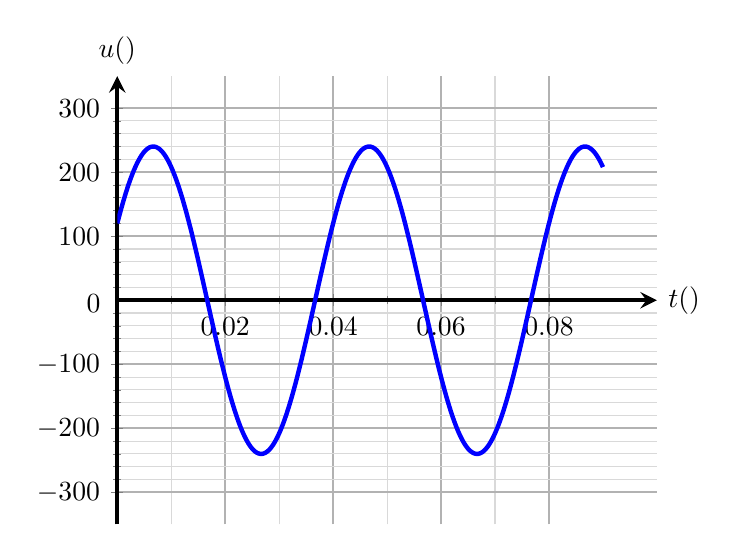
\begin{tikzpicture}  
				\begin{axis}[  ultra thick,
					xmin=0,  
					xmax=0.1,  
					xtick={0,0.02,...,0.08},
					ytick={-300,-200,...,300},
					minor x tick num=1,
					minor y tick num=4,
					ymin=-350,  
					ymax=350, 
					samples=300,
					xticklabel style={/pgf/number format/.cd, fixed,
						fixed zerofill, precision=2}, %số chữ số thập phân
					axis lines=center, 
					grid style={step=1, line width =0.4pt, color=gray!30!white},
					grid=both, %giới hạn ô lưới
					major grid style={line width=0.8pt,gray!60!white},
					xlabel=$\xsi{t}{\left(\si{\second}\right)}$, 		ylabel=$\xsi{u}{\left(\si{\volt}\right)}$,
					every axis y label/.style={at=(current axis.above origin),anchor=south},  
					every axis x label/.style={at=(current axis.right of origin),anchor=west},  ]
					\addplot [ultra thick, blue, smooth, domain=0:0.09] {240*cos(deg(50*pi*x-pi/3))};   
				\end{axis} 
				\node at (-0.3,2.8) {0}; 
			\end{tikzpicture}
			& 
			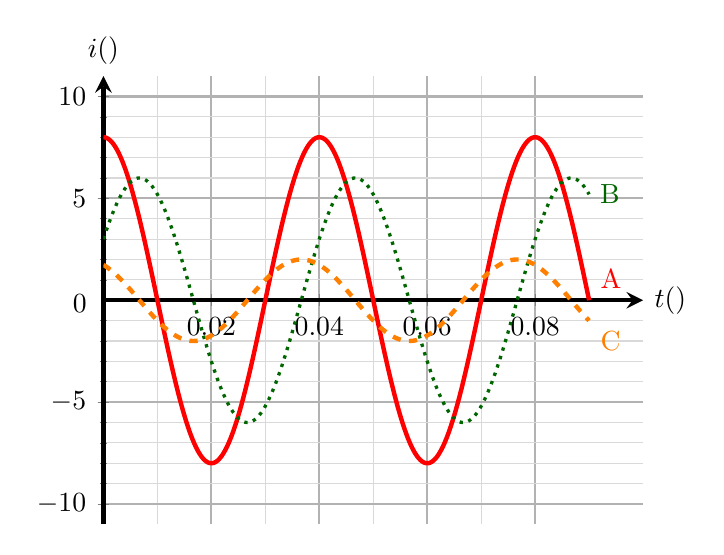
\begin{tikzpicture}  
				\begin{axis}[  ultra thick,
					xmin=0,  
					xmax=0.1,  
					xtick={0,0.02,...,0.08},
					ytick={-10,-5,...,10},
					minor x tick num=1,
					minor y tick num=4,
					ymin=-11,  
					ymax=11, 
					samples=300,
					xticklabel style={/pgf/number format/.cd, fixed,
						fixed zerofill, precision=2}, %số chữ số thập phân
					axis lines=center, 
					grid style={step=1, line width =0.4pt, color=gray!30!white},
					grid=both, %giới hạn ô lưới
					major grid style={line width=0.8pt,gray!60!white},
					xlabel=$\xsi{t}{\left(\si{\second}\right)}$, 		ylabel=$\xsi{i}{\left(\si{\ampere}\right)}$,
					every axis y label/.style={at=(current axis.above origin),anchor=south},  
					every axis x label/.style={at=(current axis.right of origin),anchor=west},  ]
					\addplot [ultra thick, red, smooth, domain=0:0.09] {8*cos(deg(50*pi*x))} node[red, above right] {A};   
					\addplot [very thick, green!40!black, smooth,dotted, domain=0:0.09] {6*cos(deg(50*pi*x-pi/3))} node[green!40!black, right] {B}; 
					\addplot [ultra thick, orange, smooth,dashed, domain=0:0.09] {2*cos(deg(50*pi*x+pi/6))} node[orange, below right] {C}; 
				\end{axis} 
				\node at (-0.3,2.8) {0}; 
			\end{tikzpicture}\\
			a) & b)
		\end{tabular}
		\captionof{figure}{}
		\label{fig: 23P-1}
	\end{center}
	Chỉ ra phát biểu \textbf{sai}.
	\choice
	{Tần số của điện áp xoay chiều và tần số của cường độ dòng điện trong ba đoạn mạch (A), (B), (C) là $\SI{25}{\hertz}$}
	{\True Pha ban đầu của cường độ dòng điện trong ba đoạn mạch (A), (B), (C) lần lượt là $\SI{0}{\radian}$, $\xsi{\dfrac{\pi}{3}}{\radian}$, $\xsi{\dfrac{\pi}{6}}{\radian}$}
	{Đoạn mạch (B) chỉ chứa điện trở thuần và có giá trị $R=\SI{40}{\ohm}$}
	{Cường độ dòng điện trong mạch điện (C) vuông pha với điện áp xoay chiều}
	\loigiai{
		Tần số của điện áp xoay chiều và tần số của cường độ dòng điện trong ba đoạn mạch (A), (B), (C) là:
		$$
		f=\dfrac{1}{T}=\frac{1}{0,04}=\SI{25}{\hertz}.
		$$
		Pha ban đầu của điện áp xoay chiều và cường độ dòng điện trong ba đoạn mạch (A), (B), (C) lần lượt là: $\varphi_{\mathrm{u}}=\xsi{-\dfrac{\pi}{3}}{\radian}$, $\varphi_{i(A)}=\SI{0}{\radian}$, $\varphi_{i(B)}=\xsi{-\dfrac{\pi}{3}}{\radian}$, $\varphi_{i(c)}=\xsi{\dfrac{\pi}{6}}{\radian}$.\\
		Cường độ dòng điện và điện áp xoay chiều trong đoạn mạch (B) dao động cùng pha với nhau nên mạch chỉ chứa điện trở thuần và có giá trị:
		$$
		R=\frac{U_0}{I_0}=\frac{240}{6}=\SI{40}{\ohm}.
		$$	
	}
\end{ex}
% ===================================================================
\begin{ex}
	Một máy phát điện xoay chiều có rôto là nam châm vĩnh cửu quay với tần số $f\ \left(\si{\text{vòng}/\second}\right)$ tạo ra trong cuộn dây trên stato một dòng điện hình sin. Mắc hai đầu cuộn dây với vôn kế để khảo sát suất điện động trong cuộn dây theo tần số quay của rôto. Kết quả được biểu diễn bằng đồ thị có trục tung là suất điện động $\xsi{E}{\left(\volt\right)}$, trục hoành là tần số quay của rôto theo đơn vị vòng/s (Hình \ref{fig: 23P-5}). Biết khi rôto không quay thì suất điện động hai đầu cuộn dây bằng 0, sai số của suất điện động là $\Delta E= \pm \SI{0.005}{\volt}$. Biểu thức nào sau đây biểu diễn mối liên hệ của suất điện động cực đại theo tần số quay của rôto?
	\begin{center}
		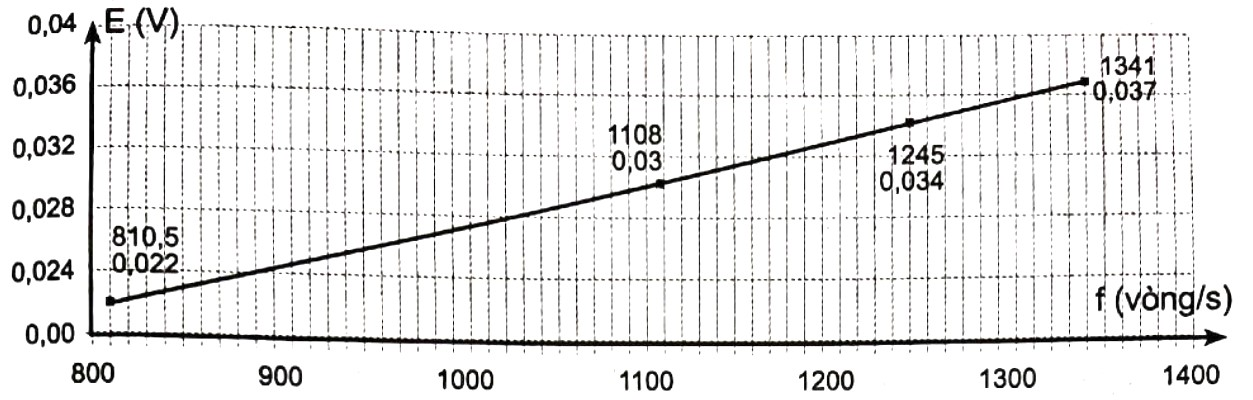
\includegraphics[width=0.85\linewidth]{figs/VN12-Y24-PH-SYL-023P-5}
		\captionof{figure}{}
		\label{fig: 23P-5}
	\end{center}
	\choice
	{\True $E_0=\xsi{3,90\cdot10^{-5}f\pm0,005}{\left(\volt\right)}$}
	{$E_0=\xsi{4,24\cdot10^{-3}f\pm0,005}{\left(\volt\right)}$}
	{$E_0=\xsi{3,01\cdot10^{-3}f\pm0,005}{\left(\volt\right)}$}
	{$E_0=\xsi{3,01\cdot10^{-3}f\pm0,005}{\left(\volt\right)}$}
	\loigiai{
		Hệ số góc của đường thẳng $E_0\left(f\right)$ là 
		$$\alpha=\dfrac{\Delta E_{0}}{\Delta f}=\dfrac{\left(\SI{0.03}{\volt}-\SI{0.022}{\volt}\right)\sqrt{2}}{\SI{1108}{\text{vòng}/\second}-\SI{810.5}{\text{vòng}/\second}}\approx\SI{3.80E-5}{\volt\cdot\second/\text{vòng}}.$$
	}
\end{ex}
% ===================================================================
\begin{ex}
	Trong máy phát điện xoay chiều có thể thay đổi số vòng dây trên stato. Khi rôto là nam châm vĩnh cửu quay làm máy hoạt động tạo ra dòng điện xoay chiều hình sin trong cuộn dây. Suất điện động $\xsi{E}{\left(\volt\right)}$ đo được ở hai đầu cuộn dây theo số vòng dây $N$ của nó có đồ thị như hình \ref{fig: 23P-6}.
	\begin{center}
		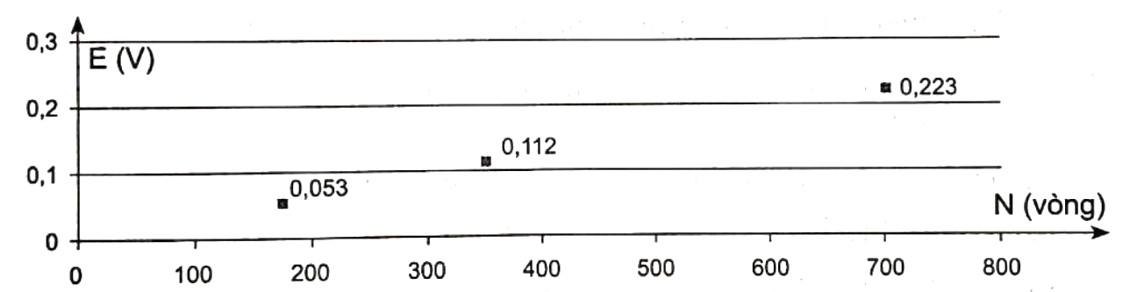
\includegraphics[width=0.7\linewidth]{figs/VN12-Y24-PH-SYL-023P-6}
		\captionof{figure}{}
		\label{fig: 23P-6}
	\end{center}
	Biểu thức nào sau đây mô tả gần đúng mối liên hệ giữa suất điện động $E$ của cuộn dây với số vòng dây $N$ (vòng) của nó?
	\choice
	{$\xsi{E}{\left(\milli\volt\right)}=53N$}
	{$\xsi{E}{\left(\volt\right)}=0,466N$}
	{\True $\xsi{E}{\left(\milli\volt\right)}=0,32N$}
	{$\xsi{E}{\left(\volt\right)}=0,112N$}
	\loigiai{
		Tính các tỉ số $\dfrac{E}{N}$ ta thấy $\xsi{E}{\left(\milli\volt\right)}=0,32N\ \left(\si{\text{vòng}}\right)$.
	}
\end{ex}
% ===================================================================
\begin{ex}
	Một đoạn mạch điện xoay chiều chỉ có điện trở thuần với giá trị $\SI{200}{\ohm}$. Đặt hiệu điện thế $\xsi{100\sqrt{2}\cos100\pi t}{\left(\volt\right)}$ vào hai đầu đoạn mạch trên thì
	\choice
	{cường độ dòng điện chạy trong mạch có giá trị hiệu dụng bằng $\xsi{\sqrt{2}}{\ampere}$}
	{dòng điện chạy trong mạch có tần số $\SI{100}{\hertz}$}
	{công suất toả nhiệt trên điện trở bằng $\SI{200}{\watt}$}
	{\True cường độ dòng điện chạy trong mạch có giá trị hiệu dụng bằng $\SI{0.5}{\ampere}$}
	\loigiai{}
\end{ex}



\Closesolutionfile{ans}
\subsubsection{Trắc nghiệm đúng/sai}
\setcounter{ex}{0}
\Opensolutionfile{ans}[ans/VN12-Y24-PH-SYL-023P-TF]
% ===================================================================
\begin{ex}
	Trong mỗi phát biểu sau, em hãy chọn đúng hoặc sai.
	\choiceTFt
	{\True Dòng điện xoay chiều giúp giảm hao phí điện năng khi truyền tải đi xa}
	{Dòng điện xoay chiều không làm toả nhiệt trên các linh kiện điện tử}
	{Điện áp hiệu dụng và cường độ dòng điện hiệu dụng của dòng điện xoay chiều có độ lớn thay đổi theo thời gian}
	{Khác với dòng điện không đổi, khi sử dụng dòng điện xoay chiều, có các điện tích tự do đi xuyên qua lớp điện môi của tụ điện}
	{Cả dòng điện không đổi và dòng điện xoay chiều đều được tăng giá trị điện áp thông qua việc sử dụng máy biến áp tăng áp có nguyên lí hoạt động dựa trên hiện tượng cảm ứng điện từ}
	{\True Mạng điện dân dụng ở nước ta sử dụng dòng điện xoay chiều có giá trị hiệu dụng $\SI{220}{\volt}$}
	{\True Dòng điện xoay chiều làm điện trở toả nhiệt như dòng điện một chiều}
	\loigiai{}
\end{ex}
% ===================================================================
\begin{ex}
	Đồ thị hình \ref{fig: 23P-2} biểu diễn từ thông và suất điện động xoay chiều trong khung dây của một máy phát điện xoay chiều.
	\begin{center}
		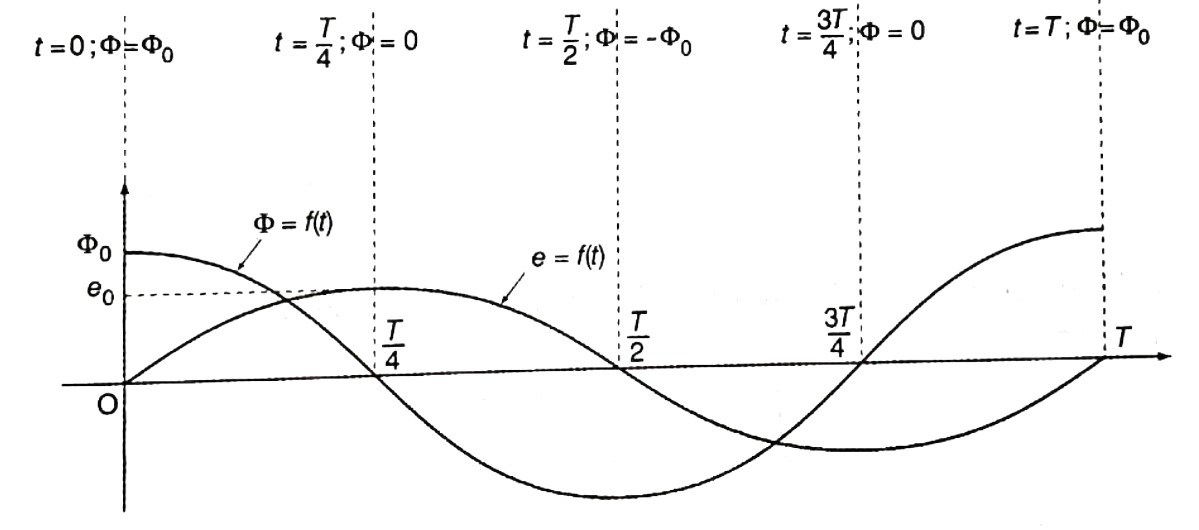
\includegraphics[width=0.65\linewidth]{figs/VN12-Y24-PH-SYL-023P-2}
		\captionof{figure}{}
		\label{fig: 23P-2}
	\end{center}
	Nhận định tính đúng hay sai của các phát biểu sau đây.
	\choiceTF[t]
	{Pha ban đầu của từ thông là $\xsi{\dfrac{\pi}{2}}{\radian}$}
	{Pha ban đầu của suất điện động biểu diễn dưới dạng hàm $\sin$ là $\xsi{\dfrac{\pi}{2}}{\radian}$}
	{\True Độ lệch pha giữa suất điện động và từ thông có độ lớn là $\xsi{\dfrac{\pi}{2}}{\radian}$}
	{\True Tại những thời điểm từ thông có trị số bằng 0 thì giá trị của suất điện động là lớn nhất}
	\loigiai{}
\end{ex}
% ===================================================================
\begin{ex}
	Một khung dây dẫn phẳng có $N$ vòng, diện tích mỗi vòng là $S$, có thể quay đều với tần số góc $\omega$ quanh trục $\Delta$ như hình $\ref{fig: 23P-3}$. Biết tại thời điểm $t=\SI{0}{\second}$ thì góc $\alpha=\SI{0}{\radian}$ và khung dây được nối với điện trở $R$ thành mạch điện kín.
	\begin{center}
		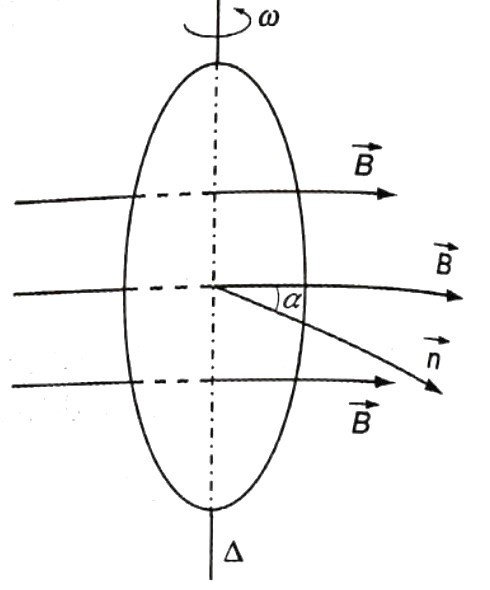
\includegraphics[width=0.3\linewidth]{figs/VN12-Y24-PH-SYL-023P-3}
		\captionof{figure}{}
		\label{fig: 23P-3}
	\end{center}
	Các nhận định sau đây là đúng hay sai?
	\choiceTF[t]
	{\True Tần số dòng điện xoay chiều qua điện trở $R$ là $f=\dfrac{\omega}{2\pi}$}
	{Suất điện động cảm ứng ở hai đầu khung dây có dạng là $e_c=\omega NBS\cos\left(\omega t+\dfrac{\pi}{2}\right)$}
	{\True Cường độ dòng điện cực đại qua điện trở $R$ là $I_0=\frac{\omega NBS}{R}$}
	{\True Độ lệch pha giữa điện áp đặt vào hai đầu điện trở và cường độ dòng điện qua điện trở là $\SI{0}{\radian}$}
	\loigiai{}
\end{ex}
% ===================================================================
\begin{ex}
	Quan sát mô hình máy phát điện xoay chiều được mô tả như hình \ref{fig: 23P-4}. Biết khung dây ABCD quay theo chiều MPNQ trong từ trường đều.
	\begin{center}
		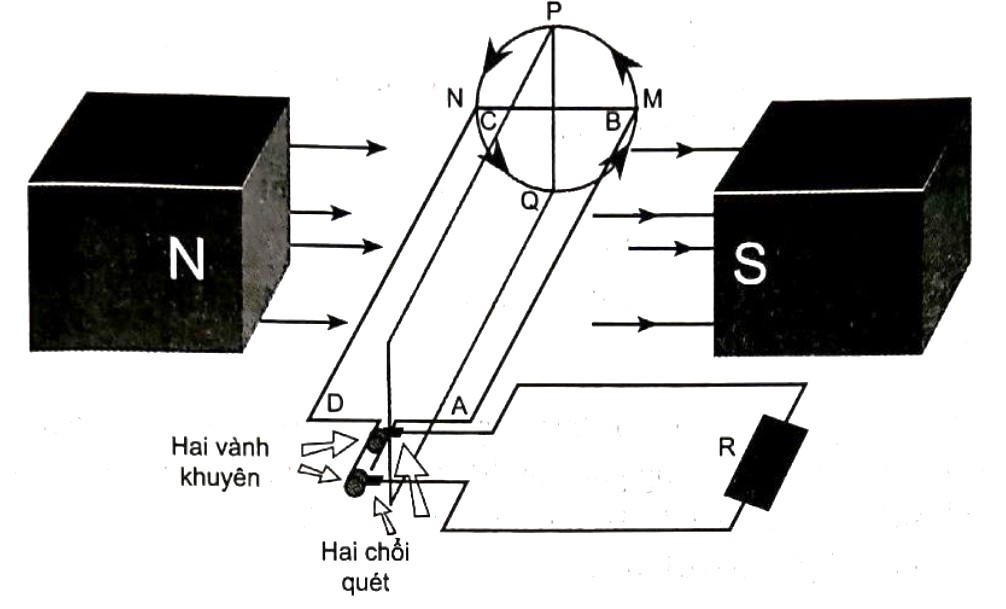
\includegraphics[width=0.5\linewidth]{figs/VN12-Y24-PH-SYL-023P-4}
		\captionof{figure}{}
		\label{fig: 23P-4}
	\end{center}
	Các nhận định sau đây là đúng hay sai?
	\choiceTF[t]
	{\True Vị trí của khung dây ABCD hiện tại có dòng điện chạy theo chiều từ A đến B}
	{\True Khi BC quay đến vị trí PQ thì chiều dòng điện chạy theo cạnh BC có hướng từ P đến Q}
	{\True Trong quá trình điểm B di chuyển từ M đến P thì cường độ dòng điện tức thời giảm}
	{\True Dòng điện đổi chiều khi BC có vị trí trùng với đường thẳng PQ}
	\loigiai{}
\end{ex}
% ===================================================================
\begin{ex}
	Quan sát mô hình máy phát điện xoay chiều được mô tả như hình \ref{fig: 23P-4}. Biết khung dây ABCD quay theo chiều MPNQ trong từ trường đều.\\
	Các nhận định sau đây về suất điện động cảm ứng xuất hiện trong khung dây là đúng hay sai? Biết suất điện động có giá trị cực đại ở vị trí của khung dây hiện tại.
	\choiceTF[t]
	{\True Quá trình điểm B di chuyển từ M đến P thì suất điện động trên khung dây đang giảm}
	{Khung dây có phương sao cho cạnh BC trùng với phương PQ thì suất điện động có giá trị âm}
	{Cạnh BC của khung dây trùng với phương MN thì suất điện động luôn có giá trị dương}
	{\True Quá trình khung dây quay có điểm B di chuyển từ Q đến M thì suất điện động đang tăng}
	\loigiai{}
\end{ex}

\Closesolutionfile{ans}
\subsubsection{Tự luận}
\setcounter{ex}{0}
\Opensolutionfile{ans}[ans/VN12-Y24-PH-SYL-023P-TL]
% ======================================================================
\begin{ex}
	Đặt điện áp xoay chiều có biểu thức $u=220\sqrt{2}\cos\left(100\pi t\right)\ \left(\si{\volt}\right)$ vào một đoạn mạch chứa các linh kiện điện tử. Biểu thức cường độ dòng điện $i=5\cos\left(100\pi t+\dfrac{\pi}{12}\right)\ \left(\si{\ampere}\right)$. Tính độ lệch pha giữa điện áp và cường độ dòng điện.
	\loigiai{
		Độ lệch pha giữa điện áp và cường độ dòng điện là $\Delta\varphi=\xsi{\dfrac{\pi}{12}}{\radian}$.
	}
\end{ex}
% ======================================================================
\begin{ex}
	Cường độ dòng điện xoay chiều qua một đoạn mạch có biểu thức $i=\cos\left(20\pi t+\dfrac{\pi}{6}\right)\ \left(\si{\milli\ampere}\right)$. Hãy xác định cường độ dòng điện tại thời điểm ban đầu.
	\loigiai{
		Tại thời điểm ban đầu ứng với $t=\SI{0}{\second}$, ta có $i\approx\SI{0.87}{\milli\ampere}$.
	}
\end{ex}
% ======================================================================
\begin{ex}
	Mạng điện xoay chiều dân dụng ở Việt Nam có tần số $\SI{50}{\hertz}$. Hãy xác định số lần dòng điện đổi chiều trong 1 giây.
	\loigiai{
		Trong một chu kì, dòng điện đổi chiều 2 lần. Một giây tương ứng với 50 chu kì, do đó dòng điện sẽ đổi chiều 100 lần.
	}
\end{ex}
% ======================================================================
\begin{ex}
	Một khung dây dẫn có diện tích $\SI{50}{\centi\meter^2}$ gồm 500 vòng dây quay đều với tốc độ $\SI{2000}{\text{vòng}/\minute}$ trong một từ trường đều $\vec{B}$ có phương vuông góc với trục quay của khung và có độ lớn cảm ứng từ $\SI{0.02}{\tesla}$. Giá trị cực đại của suất điện động cảm ứng trong khung dây là bao nhiêu?
	\loigiai{
		Giá trị cực đại của suất điện động cảm ứng là:
		$$E_0=NBS\omega=500\cdot0,02\cdot0,005\cdot2\pi\cdot\dfrac{2000}{60}\approx\SI{10.47}{\volt}.$$	
	}
\end{ex}

% ======================================================================
\begin{ex}
	Một điện áp xoay chiều được đặt vào hai đầu của một điện trở có giá trị $\SI{100}{\ohm}$. Nhiệt lượng mà điện trở toả ra trong 5 phút là $\SI{3600}{\joule}$. Điện áp cực đại có giá trị là bao nhiêu?
	\loigiai{
		Điện áp hiệu dụng đặt vào hai đầu điện trở:
		$$Q=\dfrac{U^2}{R}t\Rightarrow U=\sqrt{\dfrac{QR}{t}}=\xsi{20\sqrt{3}}{\volt}.$$
		Điện áp cực đại đặt vào hai đầu điện trở:
		$$U_0=U\sqrt{2}=\xsi{20\sqrt{6}}{\volt}\approx\SI{49}{\volt}.$$
	}
\end{ex}
% ======================================================================
\begin{ex}
	Một khung dây dẫn phẳng, có 100 vòng dây, quay trong từ trường đều, sao cho trục quay của nó luôn vuông góc với đường sức từ, với tốc độ 180 vòng/phút. Xác định suất điện động cực đại ở hai đầu khung biết từ thông cực đại gửi qua một vòng dây có giá trị $\SI{0.01}{\weber}$.
	\loigiai{
		$$E_0=\omega N\Phi_0=180\cdot\dfrac{2\pi}{60}\cdot100\cdot0,01\approx\SI{18.8}{\volt}.$$
	}
\end{ex}
% ======================================================================
\begin{ex}
	Đồ thị biểu diễn điện áp xoay chiều chạy qua một điện trở $R=\SI{50}{\ohm}$.
	\begin{center}
		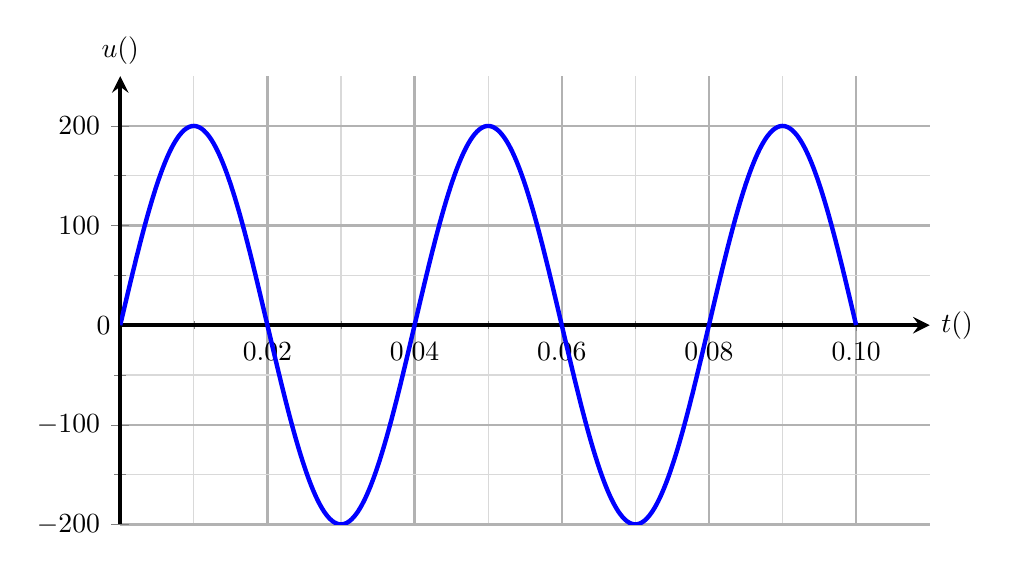
\begin{tikzpicture}  
			\begin{axis}[  ultra thick,xscale=1.5,
				xmin=0,  
				xmax=0.11,  
				xtick={0,0.02,...,0.10},
				ytick={-200,-100,...,200},
				minor x tick num=1,
				minor y tick num=1,
				ymin=-200,  
				ymax=250, 
				samples=300,
				xticklabel style={/pgf/number format/.cd, fixed,
					fixed zerofill, precision=2}, %số chữ số thập phân
				axis lines=center, 
				grid style={step=1, line width =0.4pt, color=gray!30!white},
				grid=both, %giới hạn ô lưới
				major grid style={line width=0.8pt,gray!60!white},
				xlabel=$\xsi{t}{\left(\si{\second}\right)}$, 		ylabel=$\xsi{u}{\left(\si{\volt}\right)}$,
				every axis y label/.style={at=(current axis.above origin),anchor=south},  
				every axis x label/.style={at=(current axis.right of origin),anchor=west},  ] 
				\addplot [ultra thick, blue, smooth, domain=0:0.10] {200*cos(deg(50*pi*x-pi/2))}; 
				\coordinate (O) at (axis cs:0,0);
			\end{axis} 
			\node[left] at (O) {0}; 
		\end{tikzpicture}
		
	\end{center}
	Tính:
	\begin{enumerate}[label=\alph*)]
		\item chu kì của điện áp xoay chiều;
		\item công suất tiêu thụ điện của điện trở;
		\item biểu thức của điện áp.
	\end{enumerate}
	\loigiai{
		\begin{enumerate}[label=\alph*)]
			\item Chu kì điện áp xoay chiều: $T=\SI{0.04}{\second}$.
			\item Công suất tiêu thụ điện của điện trở:
			$$\calP=\dfrac{U^2}{R}=\SI{400}{\watt}.$$
			\item Biểu thức điện áp tức thời: $u=U_0\cos\left(\omega t+\varphi_{0u}\right)$.
			\begin{itemize}
				\item Tần số góc: $\omega=\dfrac{2\pi}{T}=\xsi{50\pi}{\radian/\second}$.
				\item Điện áp cực đại: $U_0=\SI{200}{\volt}$.
				\item Pha ban đầu:\\
				Tại $t=0$ thì $u=0$ và đang tăng $\Rightarrow \varphi_{0u}=\xsi{-\dfrac{\pi}{2}}{\radian}$.
			\end{itemize}
			Thay số ta được biểu thức điện áp tức thời $u=\xsi{200\cos\left(50\pi t-\dfrac{\pi}{2}\right)}{\left(\volt\right)}$.
		\end{enumerate}	
	}
\end{ex}
% ======================================================================
\begin{ex}
	Dòng điện xoay chiều chạy qua một đoạn mạch có biểu thức $i=\xsi{2\sqrt{2}\cos\left(100\pi t\right)}{\ampere}$, $t$ tính bằng giây. Vào một thời điểm nào đó, dòng điện đang có cường độ tức thời bằng $\xsi{-2\sqrt{2}}{\ampere}$ thì sau đó ít nhất bao lâu để dòng điện có cường độ tức thời bằng $\xsi{\sqrt{6}}{\ampere}$?
	\loigiai{
		Dùng vòng tròn lượng giác thu được $\Delta t=\xsi{\dfrac{5}{600}}{\second}$.	
	}
\end{ex}
% ======================================================================
\begin{ex}
	Một khung hình vuông cạnh $a=\SI{5}{\centi\meter}$, gồm 50 vòng dây đặt trong từ trường đều có $B=\SI{0.2}{\tesla}$. Khung dây quay quanh trục với tốc độ góc $\xsi{10\pi}{\radian/\second}$ và tại $t=\SI{0}{\second}$, mặt phẳng của khung vuông góc với cảm ứng từ $\vec{B}$. Viết biểu thức suất điện động xuất hiện trong khung.
	\loigiai{
		\begin{itemize}
			\item Biểu thức của từ thông qua khung dây: $\Phi=\Phi_0\cos\left(10\pi t+\varphi_0\right)$.
			\item Với $\Phi_0=NBS=50\cdot0,2\cdot\left(\SI{5E-2}{}\right)^2=\SI{0.025}{\weber}$.
			\item Tại $t=\SI{0}{\second}$: $\varphi=\left(\vec{B}, \vec{n}\right)=\SI{0}{\radian}\Rightarrow \Phi=\xsi{0,025\cos\left(10\pi t\right)}{\weber}$.
			\item Biểu thức suất điện động xuất hiện trong khung:
			$$e_c=-\dfrac{d\Phi}{dt}=\xsi{0,785\cos\left(10\pi t-\dfrac{\pi}{2}\right)}{\left(\volt\right)}.$$
		\end{itemize}	
	}
\end{ex}

\Closesolutionfile{ans}











